\section{RESULTADOS EXPERIMENTAIS}

\subsubsection*{A. Fotodiodo}

Seguindo os passos do procedimento foi construida a Tabela \ref{tab:circ1}:

\input{r5-resultados-Table1.tex}

\subsubsection*{B. Fototransistor}

Seguindo o procedimento do item "b" do roteiro foram recolhidos os dados que constam na Tabela \ref{tab:circ2}.

% Tabela 2 - Varivolt = 60 mV e Varivolt = 80 mV
\begin{table}[!h]
    \centering
    \caption{Tensão e corrente do Fototransistor}
    \label{tab:circ2}
    \vspace{0.25cm}
    \begin{tabular}{c|cc|cc} 
        \hline
        \rule{0pt}{3ex} & \multicolumn{2}{c}{\textbf{60} [V]} & \multicolumn{2}{c}{\textbf{80} [V]} \\
        \cline{2-5} 
        \rule{0pt}{3ex}\textbf{V}$_{fonte}$ [V] & $\mathbf{V}_{D}$ [V] & $\mathbf{I}_{D}$ [A] & $\mathbf{V}_{D}$ [V] & $\mathbf{I}_{D}$ [A] \\[5pt]
        \hline
        \rule{0pt}{3ex}0.0 & 0.0 & 0.0 & 0.0 & 0.0 \\
        0.5 & 0.17 & 0.33 & 0.11 & 0.4 \\
        1.0 & 0.48 & 0.52 & 0.15 & 0.89 \\
        1.5 & 0.97 & 0.54 & 0.18 & 1.36 \\
        2.0 & 0.87 & 1.18 & 0.22 & 1.86 \\
        2.5 & 1.5 & 1.04 & 0.34 & 2.25 \\
        3.0 & 1.8 & 1.24 & 0.57 & 2.52 \\
        3.5 & 2.44 & 1.12 & 1.16 & 2.44 \\
        4.0 & 2.87 & 1.18 & 1.44 & 2.69 \\
        4.5 & 3.26 & 1.29 & 1.97 & 2.64 \\
        5.0 & 3.81 & 1.25 & 2.55 & 2.56 \\
        5.5 & 4.21 & 1.36 & 3.48 & 2.16 \\
        6.0 & 4.8 & 1.27 & 3.53 & 2.58 \\ [5pt]
        \hline
    \end{tabular}
\end{table}


\subsubsection*{C. Fotocélulas}

Para este procedimento, a professora realizou a prévia montagem do circuito conforme especificações do roteiro e foram recolhidos os dados que compoem a Tabela \ref{tab:circ3}.

% Tabela 4 - TEnsão de Circuito aberto e corrente de curto circuito da Fotocélula
\begin{table}[!h]
    \centering
    \caption{Tensão e corrente das Fotocélulas}
    \label{tab:circ3}
    \vspace{0.25cm}
    \begin{tabular}{ccc}
        \hline
        \rule{0pt}{3ex}\textbf{Entrada} & \textbf{\textbf{V}}$_{out}$ [V] & \textbf{\textbf{I}}$_{out}$ [A] \\[5pt]
        \hline
        \rule{0pt}{3ex}Escuro & 0.01 & 0 \\
        Claro & 0.41 & 0.01 \\
        60.0 V & 1.9 & 21.8 \\
        80.0 V & 2 & 46.7 \\
        100.0 V & 2.11 & 100.4 \\
        120.0 V & 2.18 & 163.0 \\
        140.0 V & 2.24 & 260 \\
        160.0 V & 2.26 & 350 \\
        180.0 V & 2.27 & 490 \\ [5pt]
        \hline
    \end{tabular}
\end{table}


\subsubsection*{D. Acoplamento óptico}

Novamente com a abordagem de experimento desmonstrativo, a professora construiu um sistema rudimentar de acoplamento óptico e que foi registratado através das figuras \ref{fig:fotos1}, \ref{fig:fotos2} e \ref{fig:fotos3}.

% Foto 1 do ociloscópio
\begin{figure}[h]
\centering
\fbox{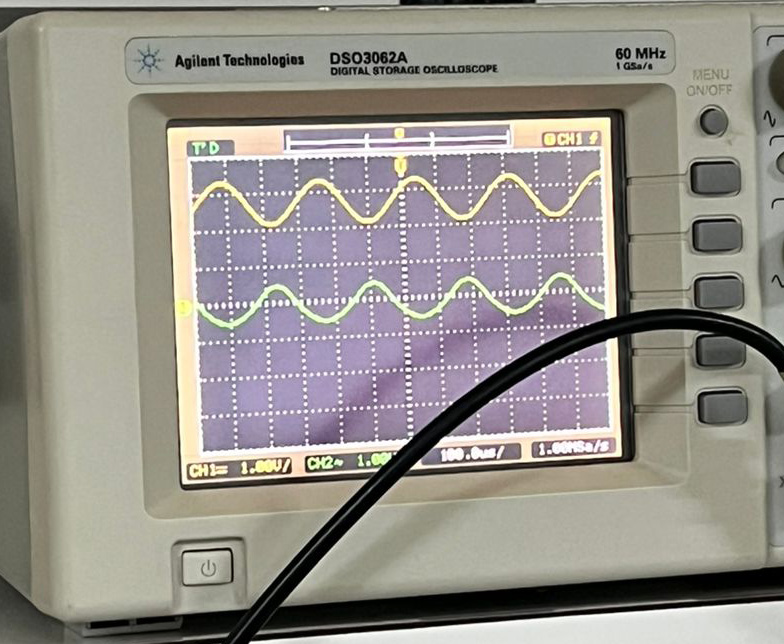
\includegraphics[width=5cm]{fotos/1.jpeg}}
\caption{Modulação e Polarização}
\label{fig:fotos1}
\end{figure}

% Foto 2 do ociloscópio
\begin{figure}[h]
\centering
\fbox{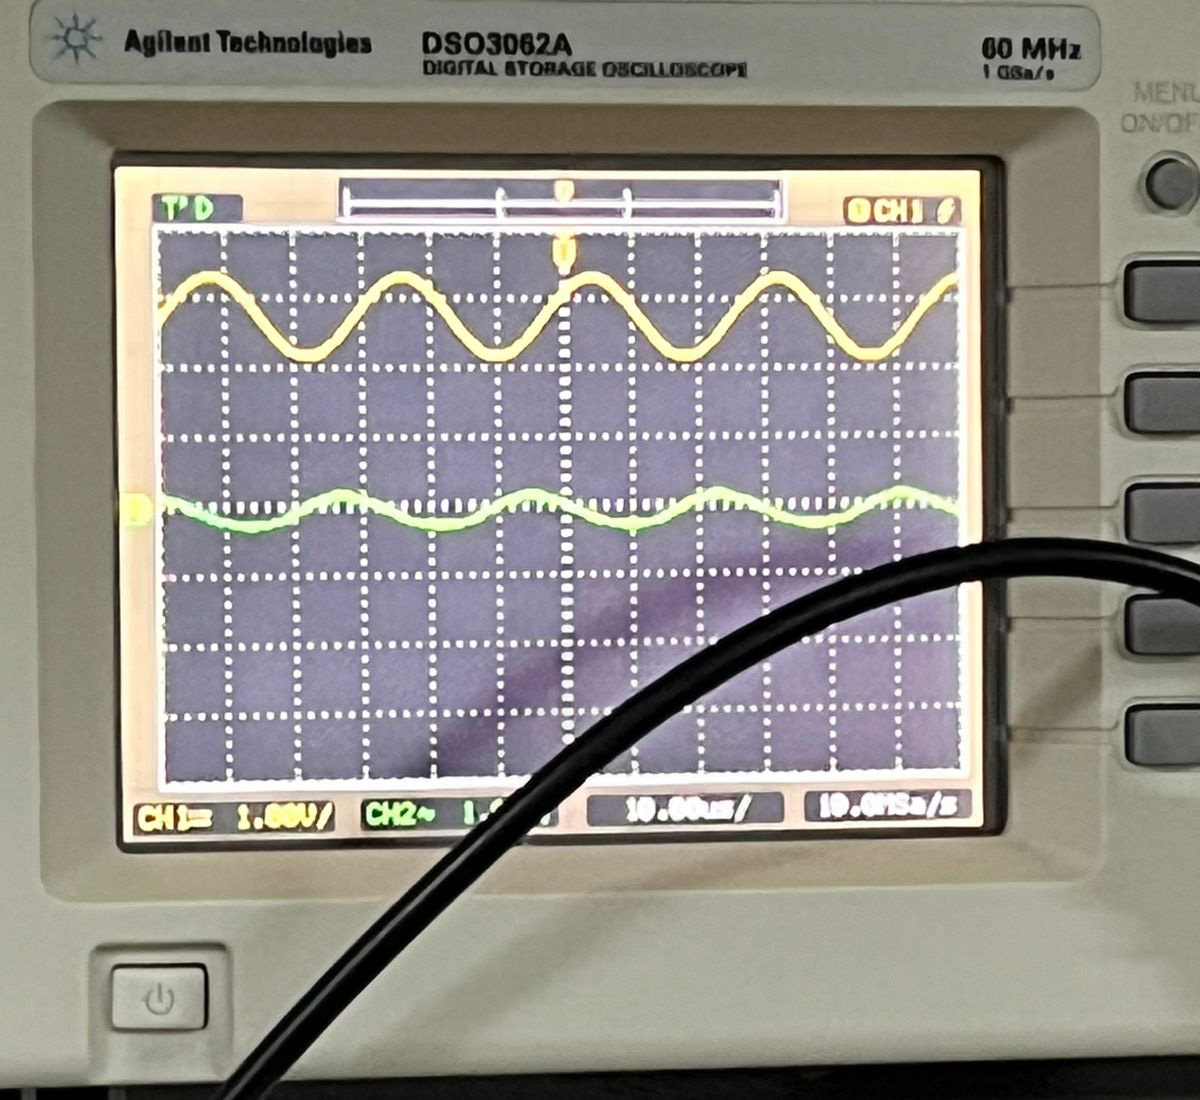
\includegraphics[width=5cm]{fotos/2.jpeg}}
\caption{Defasagem e Inversão de Fase}
\label{fig:fotos2}
\end{figure}

% Foto 3 do ociloscópio
\begin{figure}[h]
\centering
\fbox{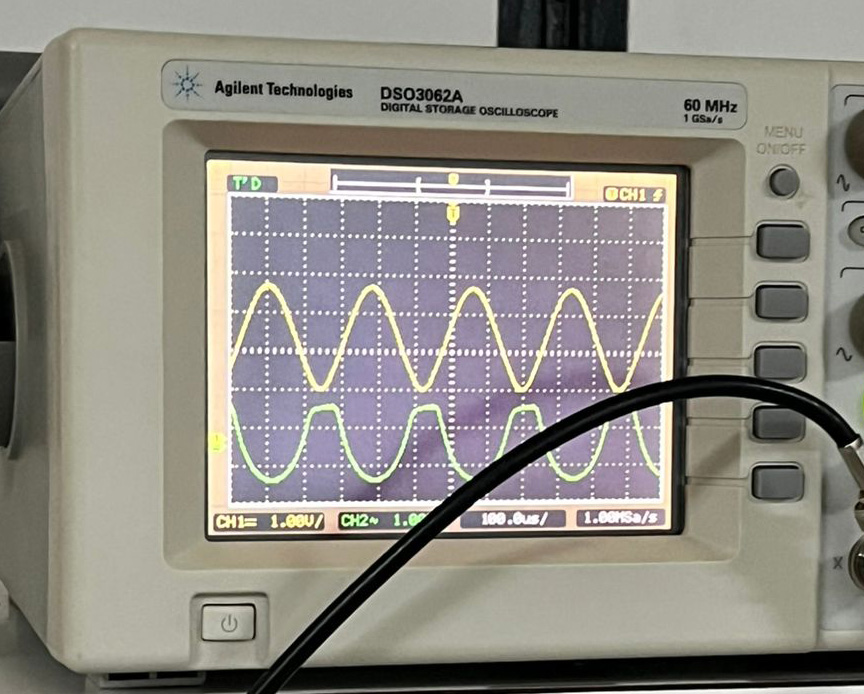
\includegraphics[width=5cm]{fotos/3.jpeg}}
\caption{Saturação e Corte}
\label{fig:fotos3}
\end{figure}

\vspace{.25cm}